\chapter{Design: A Unified Windowing System}
\label{sec:design}
The core goal of this thesis is to demonstrate, both conceptually and practically, that windowing systems are capable of solving the same problems for 3D user interfaces that they currently solve for 2D user interfaces, that a single windowing system can solve the same problems for 2D and 3D interfaces, and that a system which does so can be built on top of an existing windowing system. To understand this further, let's examine abstractly the services that a windowing system provides and how these map onto 3D interfaces.

\section{Windowing System Services}

In general, windowing systems provide a software platform for graphical applications that gives these applications a means to use the hardware resources they need to provide graphical interfaces without needing to interact with the hardware directly. Because the windowing system handles the direct interactions with the hardware, it is able to multiplex the use of hardware resources between many individual applications which need the capabilities the hardware provides. Because providing these hardware capabilities to applications abstractly is the core purpose of the windowing system, it is important to understand what it is that these hardware capabilities represent.

\subsection{Graphical Interface Hardware and The Graphical Interface Space}

Consider the interface hardware needed to provide a traditional, two dimensional, WIMP interface (and thereby needed to support a traditional windowing system). There are three essential components: a display, a mouse, and a keyboard. The display provides a two dimensional space in which two dimensional images can be drawn, and  the mouse allows limited symbolic input at any point in this two dimensional space. Together these two devices create a two dimensional spatial interface, two dimensional input and output in the same two dimensional space. 

The extension of this concept to three dimensions requires the ability of the hardware system to support three dimensional input and three dimensional output in the same three dimensional space, creating a proper three dimensional spatial interface. Immersive 3D displays provide the user with a compelling illusion of a three dimensional space which the computer can fill with arbitrary 3D content, and 3D input devices can be used to provide 3D input in this space, so existing, consumer grade 3D interface hardware can provide such a 3D interface space in the same way that a mouse and traditional display provide a 2D interface space. If the choice of 3D input device is restricted to hand held tracking devices with buttons, like the Razer Hydra used in the implementation presented here, then the 3D input set it provide is very closely analogous to the 2D input set provided by a traditional mouse: symbolic input from a few buttons coupled with continuous spatial tracking throughout the interface space.

The keyboard allows the user to give the computer complex symbolic input, but there is no spatial information attached to this input, and it is up to the software system to determine which region of the interface space, if any, that this input is delivered to. The keyboard itself is not related to the number of dimensions (or any other aspect) of the interface space, and this means that it can continue to serve its purpose in a 3D interface without needing to undergo any changes to its hardware design.

\subsection{Interface Contexts Within the Graphical Interface Space}
In a traditional windowing system, each application is given its own 2D interface space, called a window, with the same basic properties as the top level interface space provided by the hardware. An application can draw arbitrary content into its window, and receive 2D input events at any points within its bounds, giving the application a context in which it can create any 2D interface that it pleases. 

\subsubsection{Three Dimensional Interface Contexts}

Like the interface space it exists in, the concept of a window as a rectangular region of a rectangular 2D interface also has natural extensions to three dimensions. Each application can  be given a 3D region of the 3D interface space which it can fill with whatever 3D content it likes, and the system can deliver 3D input events at any location and orientation within this region. The implementation of this behaviour, especially on top of windowing infrastructure designed for 2D interfaces, has many subtleties and is the focus of the rest of this thesis.

\begin{figure}[ht!]
\centering
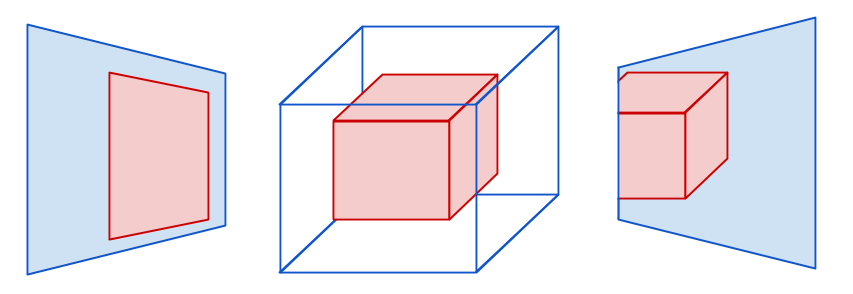
\includegraphics[width=1.0\textwidth]{images/window-types.png}
\caption{An illustration of different types of interface contexts in 3D space. From left to right: a standard 2D window with 2D content, a cuboid window with its 3D content (the red cube) embedded directly in the interface space, and a portal window, demonstrating how its 3D content is only visible through the window surface, much like a physical window.}
\end{figure}

However, unlike the extension of the interface space to 3D, which has a relatively straightforward interpretation, the interpretation of what a 3D interface context means is somewhat divergent, and requires a more in-depth analysis of what we understand a window to be. There are at least three ways to interpret the concept of a window, and each has a different extension to 3D space.

\paragraph{Cuboid Bounded}

The first interpretation regards a window as a region on the 2D interface space, a piece carved out of a whole. The extension of this interpretation to three dimensions is conceptually simple, requiring only that each application be given a box-shaped (cuboid) region of the space in which it can draw its 3D content. This type of 3D window is referred to here from here on as a cuboid window.

\paragraph{Portal-Like}

The second interpretation of the window is as a connection between one two dimensional interface space (the windowing space) and another (the application space), which more closely reflects the physical concept of a window that the window metaphor is modelled after. The extension of this interpretation to three dimensions is perhaps even more natural, since the physical concept of a window is itself three dimensional, comprising of a 2D opening which connects two physically disjoint 3D spaces into a single continuous 3D space. This requires that the clients be given the ability ability to draw content in an essentially unbounded space, but that the contents of that space can only be seen by the user through a bounded two dimensional opening, with the surface behaving as a two dimensional portal between disjoint three dimensional spaces. This type of 3D window is referred to here from here on as a portal window.

\paragraph{Unbounded}

The final interpretation is not really a separate interpretation, but rather an extension of the concept of a full screen window to the other two interpretations. In a 2D windowing system, when an application creates a full screen window it is given the ability to draw whatever content it like to every pixel on the screen, essentially being given full control of the entire interface space. Applying this concept to the other two interpretations yields interestingly convergent results. If the bounds of the cuboid window are extended to infinity, allowing it to fill the entire interface space, and if the portal through which the portal window is seen is stretched to cover the entire compositor buffer, then the application which controls these windows is able to draw content in any portion of the 3D interface space. This type of 3D window is referred to here from here on as an unbounded 3D window.

\paragraph{Correct Interpretation}

At this point the reader may be wondering which of these interpretations is correct, and if so they are encouraged to keep in mind that nothing requires that there be only one correct interpretation. Different 3D applications can have very diverse needs, and different types of 3D windows may meet these needs differently, so it could be advantageous to support all three. As discussed in Section~\ref{sec:clipping}, the way the ability of the compositor to handle all of these window types requires only minor extensions to the same core functionality, so it is possible to simply allow clients to choose which type of 3D window they wish to create.
 
\subsubsection{Two Dimensional Interface Contexts}

It is also worth noting here that because embedding a 2D surface within the 3D space is trivial (especially with the functionality provided by modern graphics APIs), it is possible for a 3D interface space to provide 2D interface contexts by simply embedding a rectangular plane in the 3D interface space and constructing a 2D interface context on the surface of this plane. Three dimensional input events can be projected onto the plane and their 2D projection can be delivered to applications as 2D input events, allowing unmodified 2D applications to use the interface space without even needing to know that it is three dimensional. Additionally, each 2D window can be given its own plane in the 3D space which can be moves, rotated, and resized independently, allowing 2D and 3D windows to be managed together in the same 3D interface space.

\section{Three Dimensional Windows With Two Dimensional Buffers}
There is a significant amount of infrastructure in place to support existing windowing systems, including established display server protocols and mechanisms for performing efficient off-screen window compositing on the GPU. Additionally, modern 3D graphics APIs like OpenGL are rich and flexible, giving application a great deal of freedom in how they use the GPU to draw their 3D content into a 2D image. All of this infrastructure, being designed to support 2D windowing systems, is designed around the idea that applications pass 2D images to the compositor, and applications which have 3D content produce a 2D image of this 3D content before doing so. While this may initially appear to be incompatible with a system which provides 3D windowing capabilities, this section is intended to illustrate that with careful design of the system allows it to take full advantage of the benefits that this infrastructure provides.

The key feature of such a design is, unsurprisingly, that it allows 3D applications to draw 2D images of their 3D content and pass these images to the windowing system, just as is done in traditional windowing systems. This design is derived from the observation that in the computer graphics pipeline, three dimensional geometric primitives (like triangles and lines) are projected to two dimensions independently and composited with one another in two dimensions to produce a 2D image of a consistent 3D space (see Section~\ref{sec:graphics-pipeline} and Section~\ref{sec:depth-perception} for more information about this process and its effect on our perception of the 3D space). The design presented here essentially seeks to coordinate this process of projection and compositing between the windowing system compositor and 3D client applications so that 3D geometry from the 3D clients can be correctly composited with the output from other 3D applications as well as geometry drawn directly by the compositor (for example surfaces for 2D clients). This creates an image of a consistent 3D scene containing geometry from multiple 3D applications without the windowing system ever needing to handle this geometry directly.

Achieving this coordination in practice is not terribly complicated, but there are several mechanisms which need to be in place for it to achieve correct, consistent results. These mechanisms are discussed here abstractly, and their implementation is discussed concretely in Section~\ref{sec:implementation}.

\subsection{Synchronized View And Projection Matrices}
As explained in Section~{sec:vertex-transform}, the view and projection matrices represent two of the transformations commonly applied to 3D geometry before it is projected onto two dimensions. The view matrix controls the apparent position of the camera, and the projection matrix controls the reduction in the apparent size of objects as they move further from the viewpoint. These transforms can be thought of as representing properties of the virtual camera (its position and optical system, respectively), and so they are applied uniformly to all geometry in the scene, reflecting the idea that the camera (and the human eye) images the scene uniformly. 

These transforms create two of the primary depth cues that give users the perception of the virtual space (discussed in detail in Section~\ref{sec:motion-parallax-and-stereopsis}), and their uniform application to all geometry in the scene is critically necessary to the ability to composite the geometric primitives which compose the scene in two dimensions. Because of this, it is necessary to ensure that the view and projection transforms applied in the compositor and the 3D clients is the same for each frame. 

\subsubsection{Buffer Size and the Projection Matrix}

In order for every 3D client to use the same projection matrices as the compositor, they must also draw into a buffer which is the same size, which incurs significant overhead when the 3D window only covers a small portion of the screen (for example when it is far away from the virtual camera). The compositor could hypothetically allocate a 2D buffer for each client which is just large enough to cover the projection of its 3D window onto the screen, but this would mean that the compositor would have to update the buffer size, projection matrix, and view matrix for each viewpoint for each client every frame, rather than only needing to update the view matrix for each viewpoint globally every frame, which significantly complicates the display server protocol extensions needed. In order to reduce the overhead, it is also possible to simply fill the stencil buffer (in both the compositor and the client) with the projection of the 3D window so that the various fragment shaders only run for pixels which lie within this projection (discussed in more detail in Section~\ref{sec:clipping}, which is the approach taken in the implementation here.

It is also hypothetically possible for the 3D clients to project their 3D geometry onto the faces of the cuboid that bounds their 3D window, or is otherwise somehow aligned with the 3D window rather than the projection plane, but this introduces texture filtering problems (as well as suffering from the multiple projection matrix problem), so it was decided against.

\subsection{Stereo Images}
Another important mechanism that informs human perception of 3D space is our ability to resolve depth from the difference in the images produced by our two eyes (see Section~\ref{sec:motion-parallax-and-stereopsis} for more details). This requires that the scene be rendered from two viewpoints (one corresponding to the position of each eye), and that these two images be sent to the correct eye. This requires that the compositor send the clients a different view and projection matrix for each viewpoint, and that the client send a separate image back to the compositor for each of these viewpoints. 

This could be accomplished with separate buffers for each eye, but in the implementation presented here, the client creates a double-wide buffer and simply writes the two images side by side in the buffer, using parameters provided by the compositor. This is discussed in more detail in Section~\ref{sec:viewpoint}.

\subsection{Depth Buffers}
\label{sec:depth-compositing}

In order for the presentation of the 3D interface to appear consistent to the user, the occlusion order of the geometry in the space must be preserved across geometry drawn by different 3D clients and by the compositor. 

One approach is to send all of the geometry to the compositor and have it draw all of the content into a 2D image (which is the approach taken by 3DWM), but this would either require that a full featured 3D graphics API be presented over the display server protocol (which would incur significant performance penalties), or it would seriously limit the flexibility clients have in producing a 2D image of their 3D scene.

The other approach, and the one taken by the system presented here, is to have the clients send their depth buffers to the compositor and composite the geometry in 2D in the same way that it is done in the traditional 3D graphics pipeline (see Section~\ref{sec:depth-test} for more information about the depth buffer and its function). This allows clients to use the graphics pipeline in any manner that they choose, and even to use completely different rendering techniques like GPU accelerated ray tracing, provided that they fill the depth buffer correctly. It also means that no new mechanism must be introduced for passing geometry to the compositor or controlling how it is drawn, which keeps the display server protocol extensions simple.

\subsection{Clipping}
\label{sec:clipping}

An important property of traditional windows is that applications can draw \textit{only} within the bounds of their window. This comes naturally with 2D windowing systems, where the application's window consists of the entire drawable area of its window buffer. However, in the system presented here, 3D clients draw into a buffer which is the same dimensions as the buffer which the compositor draws into, allowing an uncontrolled client to draw into any portion of the 3D interface space.

The solve this problem, the compositor presented here is designed to simply ignore pixels in the buffer produced by 3D clients if they lie outside the bounds of its 3D window. The exact procedure which ensures this varies depending on which type of 3D window is being clipped, and is discussed in more detail in Section~\ref{sec:clipping-impl}.